\section{Ejercicio 3}
	Se pedía crear una tarea que usara el procesador cierto tiempo (\texttt{total_cpu}) y, dentro de ese tiempo, tuviera una cantidad de bloqueos (\texttt{cant_bloqueos}). Se procedió a crear un vector donde se guardan los tiempos en que se realizarán las llamadas bloqueantes, los cuales se generan de forma aleatoria. Cada vez que se obtiene uno de ellos, se verifica que no esté repetido con los anteriores. Una vez obtenido este conjunto de tiempos, se pasa ordenarlos de menor a mayor, para luego ir creando los intervalos en los cuales el proceso usará el procesador; para esto se toma el tiempo entre dos bloqueos consecutivos. Como pedía el enunciado, cada bloqueo tiene una duración de 2 \emph{quantums}.

	\begin{figure}[ht]
		\begin{center}
			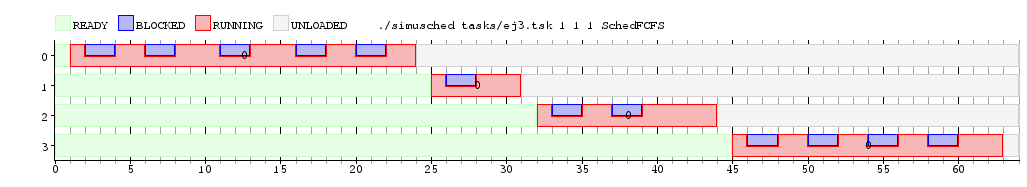
\includegraphics[width=1\columnwidth]{imagenes/ej3.png}
			\caption{\texttt{TaskBatch} corriendo con $total_cpu = 4$, $cant_bloqueos = 2$.}
		\end{center}
	\end{figure}

